
%%%%%%%%%%%%%%%%%%%%%%%%%%%%%%%%%%%%%%%%%%%%%%%%
% Appendix
%%%%%%%%%%%%%%%%%%%%%%%%%%%%%%%%%%%%%%%%%%%%%%%%

\clearpage
\section{Experimental Setup and Full Accuracy Breakdown}\label{app:setup}\label{app:ablation}

Table~\ref{tab:performance_full} provides the full per-position accuracy breakdown (Prefix, Infix, Suffix) corresponding to the best-across-positions results summarized in Table~\ref{tab:performance} in the main text. Table~\ref{tab:token_count} lists the number of RSP tokens $L$ used for each model--benchmark pair, selected from $\{10, 15, 20\}$. All experiments are conducted on a single NVIDIA A6000 40GB GPU with greedy decoding, a maximum generation length of 3{,}072 tokens for MATH-500 and GSM8K, and 4{,}096 tokens for AIME24. Batch size is fixed per model (16 for LLaMA-3.1-8B-Instruct and Qwen2.5-Math-7B variants, 32 for Qwen2.5-Math-1.5B variants).

\begin{table}[ht]
\centering
\caption{Accuracy (\%) across model configurations, injection positions, and benchmarks. Values in parentheses indicate the difference from the baseline. \textbf{Bold} denotes the best result and \underline{underline} denotes the second best for each model--benchmark pair.}
\label{tab:performance_full}
\footnotesize
\renewcommand{\arraystretch}{0.9}
\begin{tabular}{ll ccc}
\toprule
\textbf{Model} & \textbf{Mode} & \textbf{MATH-500} & \textbf{GSM8K} & \textbf{AIME24} \\
\midrule
\multicolumn{5}{l}{\textit{Instruct Models}} \\
\midrule
\multirow{4}{*}{LLaMA-3.1-8B-Instruct} & Baseline & \textbf{52.20} & 85.75 & \underline{6.67} \\
 & Prefix & 45.00 {\scriptsize($-$7.2)} & 76.35 {\scriptsize($-$9.4)} & 3.33 {\scriptsize($-$3.3)} \\
 & Infix & \underline{49.40} {\scriptsize($-$2.8)} & \underline{85.97} {\scriptsize(+0.2)} & \textbf{10.00} {\scriptsize(+3.3)} \\
 & Suffix & \underline{49.40} {\scriptsize($-$2.8)} & \textbf{86.73} {\scriptsize(+1.0)} & \textbf{10.00} {\scriptsize(+3.3)} \\
\midrule
\multirow{4}{*}{Qwen2.5-Math-7B-Instruct} & Baseline & 83.20 & 95.45 & \underline{13.33} \\
 & Prefix & 81.40 {\scriptsize($-$1.8)} & 94.92 {\scriptsize($-$0.5)} & \underline{13.33} {\scriptsize(+0.0)} \\
 & Infix & \textbf{84.20} {\scriptsize(+1.0)} & \underline{95.60} {\scriptsize(+0.2)} & \textbf{16.67} {\scriptsize(+3.3)} \\
 & Suffix & \underline{83.40} {\scriptsize(+0.2)} & \textbf{95.68} {\scriptsize(+0.2)} & \textbf{16.67} {\scriptsize(+3.3)} \\
\midrule
\multirow{4}{*}{Qwen2.5-Math-1.5B-Instruct} & Baseline & 73.00 & \underline{85.29} & 10.00 \\
 & Prefix & \underline{74.80} {\scriptsize(+1.8)} & \underline{85.29} {\scriptsize(+0.0)} & \underline{13.33} {\scriptsize(+3.3)} \\
 & Infix & \textbf{75.20} {\scriptsize(+2.2)} & \textbf{85.75} {\scriptsize(+0.5)} & 6.67 {\scriptsize($-$3.3)} \\
 & Suffix & 74.20 {\scriptsize(+1.2)} & 84.69 {\scriptsize($-$0.6)} & \textbf{20.00} {\scriptsize(+10.0)} \\
\midrule
\multicolumn{5}{l}{\textit{Base Models (Raw Text)}} \\
\midrule
\multirow{4}{*}{Qwen2.5-Math-7B} & Baseline & \textbf{72.20} & \underline{84.15} & 6.67 \\
 & Prefix & \underline{71.60} {\scriptsize($-$0.6)} & \textbf{84.31} {\scriptsize(+0.2)} & \textbf{16.67} {\scriptsize(+10.0)} \\
 & Infix & 63.20 {\scriptsize($-$9.0)} & 64.29 {\scriptsize($-$19.9)} & \textbf{16.67} {\scriptsize(+10.0)} \\
 & Suffix & 55.60 {\scriptsize($-$16.6)} & 54.13 {\scriptsize($-$30.0)} & \underline{13.33} {\scriptsize(+6.7)} \\
\midrule
\multirow{4}{*}{Qwen2.5-Math-1.5B} & Baseline & \underline{61.40} & \textbf{77.86} & \textbf{16.67} \\
 & Prefix & \textbf{64.40} {\scriptsize(+3.0)} & \underline{74.30} {\scriptsize($-$3.6)} & \underline{10.00} {\scriptsize($-$6.7)} \\
 & Infix & 63.20 {\scriptsize(+1.8)} & 73.92 {\scriptsize($-$3.9)} & \underline{10.00} {\scriptsize($-$6.7)} \\
 & Suffix & 54.60 {\scriptsize($-$6.8)} & 58.61 {\scriptsize($-$19.3)} & 3.33 {\scriptsize($-$13.3)} \\
\midrule
\multicolumn{5}{l}{\textit{Base Models + ChatML (Format Mismatch)}} \\
\midrule
\multirow{4}{*}{Qwen2.5-Math-7B} & Baseline & 52.20 & 58.30 & \textbf{23.33} \\
 & Prefix & 59.20 {\scriptsize(+7.0)} & 56.41 {\scriptsize($-$1.9)} & \underline{3.33} {\scriptsize($-$20.0)} \\
 & Infix & \underline{62.00} {\scriptsize(+9.8)} & \underline{69.07} {\scriptsize(+10.8)} & \textbf{23.33} {\scriptsize(+0.0)} \\
 & Suffix & \textbf{70.40} {\scriptsize(+18.2)} & \textbf{75.97} {\scriptsize(+17.7)} & \textbf{23.33} {\scriptsize(+0.0)} \\
\midrule
\multirow{4}{*}{Qwen2.5-Math-1.5B} & Baseline & 34.40 & 37.45 & \underline{13.33} \\
 & Prefix & \textbf{63.40} {\scriptsize(+29.0)} & \textbf{67.02} {\scriptsize(+29.6)} & \textbf{20.00} {\scriptsize(+6.7)} \\
 & Infix & 39.20 {\scriptsize(+4.8)} & 50.42 {\scriptsize(+13.0)} & 6.67 {\scriptsize($-$6.7)} \\
 & Suffix & \underline{51.00} {\scriptsize(+16.6)} & \underline{50.64} {\scriptsize(+13.2)} & \underline{13.33} {\scriptsize(+0.0)} \\
\bottomrule
\end{tabular}
\end{table}

\begin{table}[ht]
\centering
\caption{Number of RSP tokens ($L$) used for each model and benchmark.}
\label{tab:token_count}
\footnotesize
\renewcommand{\arraystretch}{0.9}
\begin{tabular}{lccc}
\toprule
\textbf{Model} & \textbf{MATH-500} & \textbf{GSM8K} & \textbf{AIME24} \\
\midrule
LLaMA-3.1-8B-Instruct & 15 & 20 & 15 \\
Qwen2.5-Math-7B-Instruct & 20 & 20 & 20 \\
Qwen2.5-Math-1.5B-Instruct & 20 & 10 & 20 \\
Qwen2.5-Math-7B & 10 & 10 & 20 \\
Qwen2.5-Math-1.5B & 10 & 10 & 20 \\
Qwen2.5-Math-1.5B (ChatML) & 20 & 20 & 10 \\
Qwen2.5-Math-7B (ChatML) & 20 & 20 & 20 \\
\bottomrule
\end{tabular}
\end{table}

% ================================================================
\subsection{RSP Injection Positions and Prompt Templates}\label{app:injection_positions}
% ================================================================

Below we show the prompt structure for each injection position across all model types. \textcolor{blue!70!black}{Blue text} indicates RSP embeddings, and \textcolor{purple}{purple text} indicates special tokens.

% --------------------------------
\subsubsection{Prefix}
% --------------------------------

RSP embeddings are concatenated before the prompt embeddings. No text modification is applied.

\paragraph{ChatML (Qwen Instruct / Base + ChatML).}
\begin{tcolorbox}[colback=gray!5, colframe=black!60, arc=3pt, boxrule=0.5pt, fontupper=\footnotesize\ttfamily, breakable]
\textcolor{blue!70!black}{[Random Embeddings ($L$ tokens)]}\\
\textcolor{purple}{<|im\_start|>}system\\
Please reason step by step, and put your final answer within \textbackslash boxed\{\}.\textcolor{purple}{<|im\_end|>}\\
\textcolor{purple}{<|im\_start|>}user\\
\{question\}\textcolor{purple}{<|im\_end|>}\\
\textcolor{purple}{<|im\_start|>}assistant
\end{tcolorbox}

\paragraph{LLaMA Chat Template.}
\begin{tcolorbox}[colback=gray!5, colframe=black!60, arc=3pt, boxrule=0.5pt, fontupper=\footnotesize\ttfamily, breakable]
\textcolor{blue!70!black}{[Random Embeddings ($L$ tokens)]}\\
\textcolor{purple}{<|begin\_of\_text|>}\\
\textcolor{purple}{<|start\_header\_id|>}system\textcolor{purple}{<|end\_header\_id|>}\\
Cutting Knowledge Date: December 2023\\
Today Date: 26 Jul 2024\\
Please reason step by step, and put your final answer within \textbackslash boxed\{\}.\textcolor{purple}{<|eot\_id|>}\\
\textcolor{purple}{<|start\_header\_id|>}user\textcolor{purple}{<|end\_header\_id|>}\\
\{question\}\textcolor{purple}{<|eot\_id|>}\\
\textcolor{purple}{<|start\_header\_id|>}assistant\textcolor{purple}{<|end\_header\_id|>}
\end{tcolorbox}

\paragraph{Raw Text (Qwen Base).}
\begin{tcolorbox}[colback=gray!5, colframe=black!60, arc=3pt, boxrule=0.5pt, fontupper=\footnotesize\ttfamily, breakable]
\textcolor{blue!70!black}{[Random Embeddings ($L$ tokens)]}\\
\{question\}\\
Please reason step by step, and put your final answer within \textbackslash boxed\{\}.
\end{tcolorbox}

% --------------------------------
\subsubsection{Infix}
% --------------------------------

A description text and special tokens are inserted into the prompt. The special token positions are then replaced with RSP embeddings at the embedding level.

\paragraph{ChatML (Qwen Instruct / Base + ChatML).}
\begin{tcolorbox}[colback=gray!5, colframe=black!60, arc=3pt, boxrule=0.5pt, fontupper=\footnotesize\ttfamily, breakable]
\textcolor{purple}{<|im\_start|>}system\\
Please reason step by step, and put your final answer within \textbackslash boxed\{\}.\textcolor{purple}{<|im\_end|>}\\
\textcolor{purple}{<|im\_start|>}user\\
\{question\}\\[0.3em]
\textcolor{gray}{There are \{$L$\} special tokens that contain compressed latent reasoning information that might be useful for your reasoning. If these tokens are useful for your case, you can use them as reference. If these tokens are not useful for your case, you can ignore them and focus back to solving the problem.}\\[0.3em]
Here are the \{$L$\} special tokens: \textcolor{blue!70!black}{<special\_token\_1>...<special\_token\_$L$>}\\
\textcolor{purple}{<|im\_end|>}\\
\textcolor{purple}{<|im\_start|>}assistant
\end{tcolorbox}

\paragraph{LLaMA Chat Template.}
\begin{tcolorbox}[colback=gray!5, colframe=black!60, arc=3pt, boxrule=0.5pt, fontupper=\footnotesize\ttfamily, breakable]
\textcolor{purple}{<|begin\_of\_text|>}\\
\textcolor{purple}{<|start\_header\_id|>}system\textcolor{purple}{<|end\_header\_id|>}\\
Cutting Knowledge Date: December 2023\\
Today Date: 26 Jul 2024\\
Please reason step by step, and put your final answer within \textbackslash boxed\{\}.\textcolor{purple}{<|eot\_id|>}\\
\textcolor{purple}{<|start\_header\_id|>}user\textcolor{purple}{<|end\_header\_id|>}\\
\{question\}\\[0.3em]
\textcolor{gray}{There are \{$L$\} special tokens that contain compressed latent reasoning information that might be useful for your reasoning. If these tokens are useful for your case, you can use them as reference. If these tokens are not useful for your case, you can ignore them and focus back to solving the problem.}\\[0.3em]
Here are the \{$L$\} special tokens:\\
\textcolor{blue!70!black}{<reserved\_special\_token\_0>...}\\
\textcolor{blue!70!black}{<reserved\_special\_token\_$L$>}\\
\textcolor{purple}{<|eot\_id|>}\\
\textcolor{purple}{<|start\_header\_id|>}assistant\textcolor{purple}{<|end\_header\_id|>}
\end{tcolorbox}

\paragraph{Raw Text (Qwen Base).}
\begin{tcolorbox}[colback=gray!5, colframe=black!60, arc=3pt, boxrule=0.5pt, fontupper=\footnotesize\ttfamily, breakable]
\{question\}\\[0.3em]
\textcolor{gray}{There are \{$L$\} special tokens that contain compressed latent reasoning information that might be useful for your reasoning. If these tokens are useful for your case, you can use them as reference. If these tokens are not useful for your case, you can ignore them and focus back to solving the problem.}\\[0.3em]
Here are the \{$L$\} special tokens: \textcolor{blue!70!black}{<special\_token\_1>...<special\_token\_$L$>}\\[0.3em]
Please reason step by step, and put your final answer within \textbackslash boxed\{\}.
\end{tcolorbox}

% --------------------------------
\subsubsection{Suffix}
% --------------------------------

For chat-templated models, RSP embeddings are inserted immediately before the end-of-turn token. For raw text models, RSP embeddings are concatenated at the end of the prompt.

\paragraph{ChatML (Qwen Instruct / Base + ChatML).}
\begin{tcolorbox}[colback=gray!5, colframe=black!60, arc=3pt, boxrule=0.5pt, fontupper=\footnotesize\ttfamily, breakable]
\textcolor{purple}{<|im\_start|>}system\\
Please reason step by step, and put your final answer within \textbackslash boxed\{\}.\textcolor{purple}{<|im\_end|>}\\
\textcolor{purple}{<|im\_start|>}user\\
\{question\}\textcolor{blue!70!black}{[Random Embeddings ($L$ tokens)]}\textcolor{purple}{<|im\_end|>}\\
\textcolor{purple}{<|im\_start|>}assistant
\end{tcolorbox}

\paragraph{LLaMA Chat Template.}
\begin{tcolorbox}[colback=gray!5, colframe=black!60, arc=3pt, boxrule=0.5pt, fontupper=\footnotesize\ttfamily, breakable]
\textcolor{purple}{<|begin\_of\_text|>}\\
\textcolor{purple}{<|start\_header\_id|>}system\textcolor{purple}{<|end\_header\_id|>}\\
Cutting Knowledge Date: December 2023\\
Today Date: 26 Jul 2024\\
Please reason step by step, and put your final answer within \textbackslash boxed\{\}.\textcolor{purple}{<|eot\_id|>}\\
\textcolor{purple}{<|start\_header\_id|>}user\textcolor{purple}{<|end\_header\_id|>}\\
\{question\}\textcolor{blue!70!black}{[Random Embeddings ($L$ tokens)]}\textcolor{purple}{<|eot\_id|>}\\
\textcolor{purple}{<|start\_header\_id|>}assistant\textcolor{purple}{<|end\_header\_id|>}
\end{tcolorbox}

\paragraph{Raw Text (Qwen Base).}
\begin{tcolorbox}[colback=gray!5, colframe=black!60, arc=3pt, boxrule=0.5pt, fontupper=\footnotesize\ttfamily, breakable]
\{question\}\\
Please reason step by step, and put your final answer within \textbackslash boxed\{\}.\textcolor{blue!70!black}{[Random Embeddings ($L$ tokens)]}
\end{tcolorbox}

% ================================================================
\subsection{Answer Extraction and Grading}\label{app:extraction}
% ================================================================

The final answer is extracted from the model output through a fallback chain. Each step is attempted in order; if extraction fails, the next step is tried.

\begin{tcolorbox}[colback=gray!5, colframe=black!60, arc=3pt, boxrule=0.5pt, title=\textbf{Answer Extraction Fallback Chain}, fonttitle=\small, coltitle=black, colbacktitle=gray!20]
\small
\begin{enumerate}[leftmargin=*, nosep]
  \item \texttt{"final answer is \$...\$. I hope"} pattern (Minerva format)
  \item \texttt{\textbackslash boxed\{...\}}: last non-empty box is used; empty \texttt{\textbackslash boxed\{\}} are skipped
  \item Text following \texttt{"the answer is"}
  \item Text following \texttt{"final answer is"}
  \item Last number in the output (regex fallback)
\end{enumerate}
\end{tcolorbox}

\vspace{0.5em}
Extracted answers are normalized by removing \texttt{\$}, \texttt{\textbackslash left}, \texttt{\textbackslash right}, and unit strings. Grading is performed via symbolic equivalence checking: exact string match, numerical comparison (\texttt{math.isclose}, \texttt{rel\_tol=1e-4}), and SymPy symbolic simplification.

% ================================================================
\subsection{Reproduced Prior Work Hyperparameters}
% ================================================================

All prior methods are reproduced on Qwen2.5-Math-1.5B-Instruct and Qwen2.5-Math-7B-Instruct, evaluated with greedy decoding (temperature $= 0$) and our unified answer extraction pipeline.

\paragraph{TTSV.} Prefix length 20, trained for 20 epochs with AdamW optimizer, batch size 2, gradient accumulation 8 steps, and linear learning rate schedule. Learning rate is 1e-3 for Qwen-1.5B and 1e-5 for Qwen-7B.

\paragraph{LTPO.} Table~\ref{tab:hp_ltpo} reports the per-benchmark hyperparameters.

\begin{table}[ht]
\centering
\caption{LTPO hyperparameters.}
\label{tab:hp_ltpo}
\footnotesize
\renewcommand{\arraystretch}{0.9}
\begin{tabular}{lccc}
\toprule
\textbf{Parameter} & \textbf{GSM8K} & \textbf{MATH-500} & \textbf{AIME24} \\
\midrule
tokens & 8 & 8 & 8 \\
steps & 20 & 20 & 20 \\
top\_k & 10 & 10 & 10 \\
sigma & 20 & 20 & 5 \\
sigma\_decay & 0.95 & 0.95 & 0.95 \\
lr & 1e-2 & 5e-3 & 5e-2 \\
\bottomrule
\end{tabular}
\end{table}

\paragraph{SoftCoT.} Projection module trained for 10 epochs. Thought tokens: 32 during training, 4 during evaluation. Batch size 4 for GSM8K, 1 for MATH with gradient accumulation 4. The small (assistant) model is Qwen2.5-Math-1.5B-Instruct in both configurations, while the large model is Qwen2.5-Math-1.5B-Instruct (learning rate 2e-5) or Qwen2.5-Math-7B-Instruct (learning rate 5e-6). For MATH-500 and AIME24 evaluation, we use the projection module trained on GSM8K, as it yields higher accuracy than the one trained on MATH.

% ================================================================
\subsection{Full Entropy Curves}\label{app:entropy_full}
% ================================================================

Figure~\ref{fig:app_full_entropy} shows the full normalized (0--100\%) generation trajectories for entropy, top-1 probability, and varentropy, and Table~\ref{tab:entropy_full} reports the corresponding scalar statistics including overall means, first-5\% means, and the average number of generated tokens per problem. All methods converge to similar levels after the initial generation stage, confirming that the distributional changes induced by RSP are localized to the early reasoning phase.

\begin{table}[ht]
\centering
\caption{Per-step statistics for Qwen2.5-Math-1.5B-Instruct on MATH-500 across the full generation and the first 5\% of generation steps, together with the average number of generated tokens per problem. Top-1 Prob (overall) is reported as a weighted average over the first-10\%/middle/last-10\% segment means with weights $0.1/0.8/0.1$. Extension of Figure~\ref{fig:entropy_first5} (main text) and Figure~\ref{fig:app_full_entropy}.}
\label{tab:entropy_full}
\footnotesize
\setlength{\tabcolsep}{4pt}
\renewcommand{\arraystretch}{0.9}
\begin{tabular}{lccccccc}
\toprule
\textbf{Metric} & \textbf{Baseline} & \cellcolor{blue!10}\textbf{Prefix} & \cellcolor{blue!10}\textbf{Infix} & \cellcolor{blue!10}\textbf{Suffix} & \textbf{LTPO} & \textbf{SoftCoT} & \textbf{TTSV} \\
\midrule
Tokens (mean)            & 575.7  & \cellcolor{blue!10}558.4  & \cellcolor{blue!10}549.9  & \cellcolor{blue!10}573.3  & 592.3  & 594.4  & 577.4  \\
\midrule
Entropy (first 5\%)      & 0.1332 & \cellcolor{blue!10}0.1366 & \cellcolor{blue!10}0.1402 & \cellcolor{blue!10}0.1941 & 0.1662 & 0.4218 & 0.1359 \\
Entropy (overall)        & 0.0871 & \cellcolor{blue!10}0.0881 & \cellcolor{blue!10}0.0899 & \cellcolor{blue!10}0.1049 & 0.0909 & 0.1059 & 0.0864 \\
\midrule
Top-1 Prob (first 5\%)   & 0.9535 & \cellcolor{blue!10}0.9523 & \cellcolor{blue!10}0.9525 & \cellcolor{blue!10}0.9373 & 0.9437 & 0.9156 & 0.9534 \\
Top-1 Prob (overall)     & 0.9684 & \cellcolor{blue!10}0.9681 & \cellcolor{blue!10}0.9678 & \cellcolor{blue!10}0.9647 & 0.9683 & 0.9651 & 0.9685 \\
\midrule
Varentropy (first 5\%)   & 0.2181 & \cellcolor{blue!10}0.2207 & \cellcolor{blue!10}0.2463 & \cellcolor{blue!10}0.4010 & 0.2953 & 2.2234 & 0.2174 \\
Varentropy (overall)     & 0.1353 & \cellcolor{blue!10}0.1375 & \cellcolor{blue!10}0.1422 & \cellcolor{blue!10}0.2038 & 0.1452 & 0.2404 & 0.1361 \\
\bottomrule
\end{tabular}
\end{table}

\begin{figure}[ht]
  \centering
  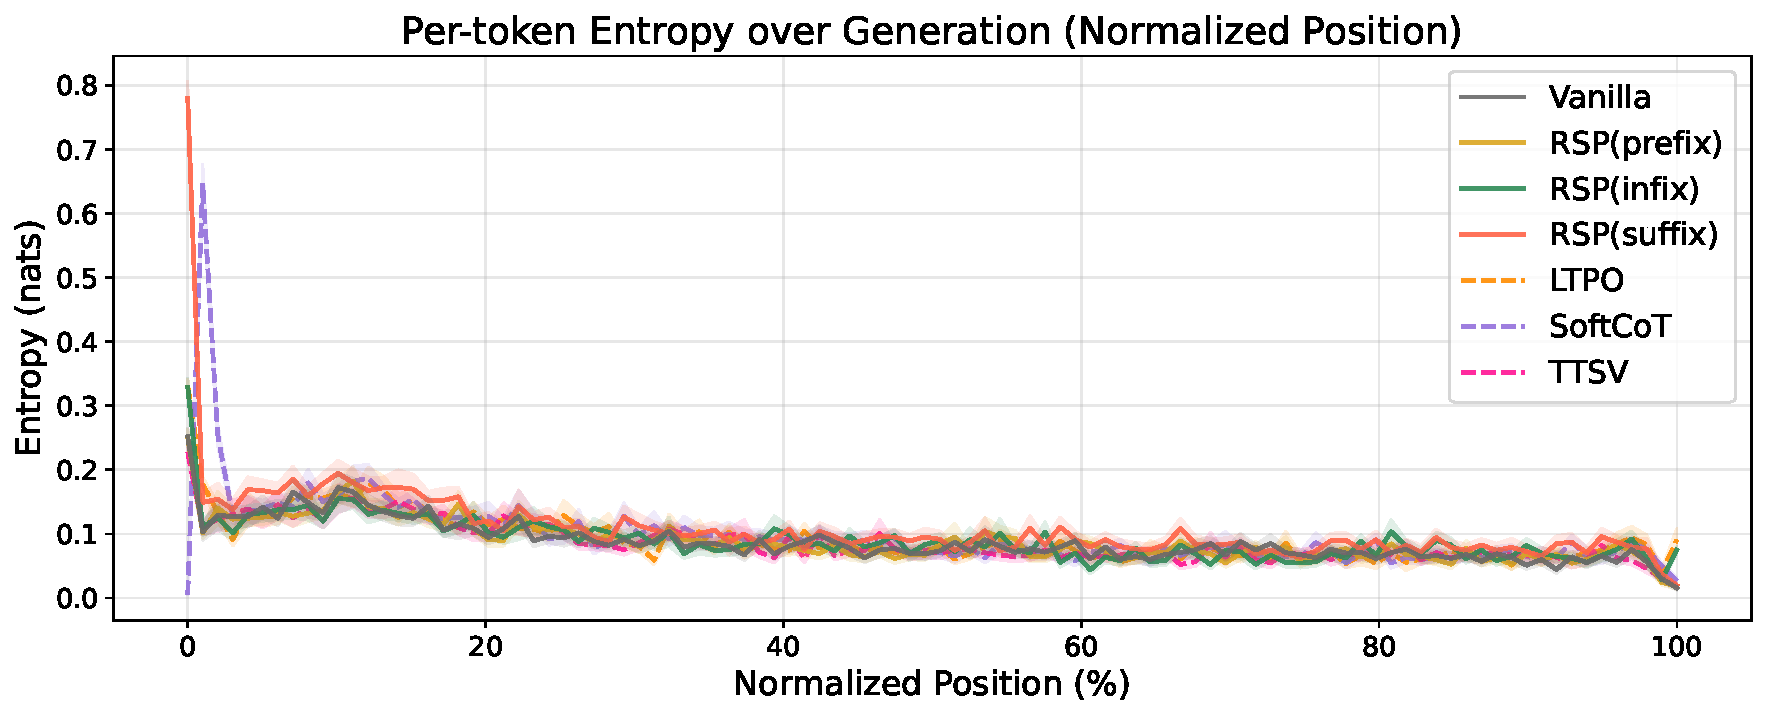
\includegraphics[width=0.85\textwidth]{img/entropy/full_entropy.pdf}\\[0.4em]
  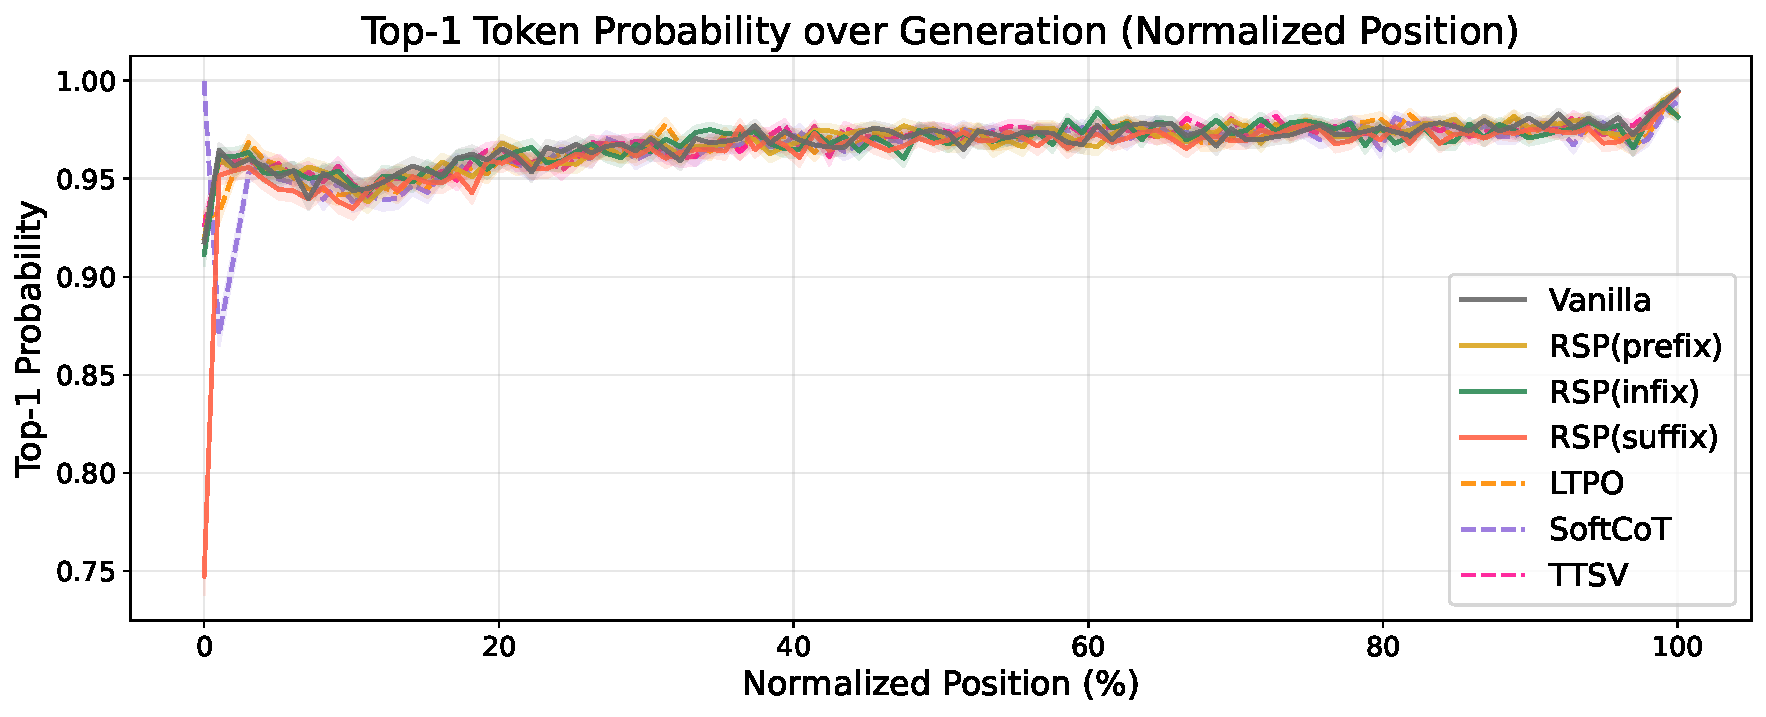
\includegraphics[width=0.85\textwidth]{img/entropy/full_top1prob.pdf}\\[0.4em]
  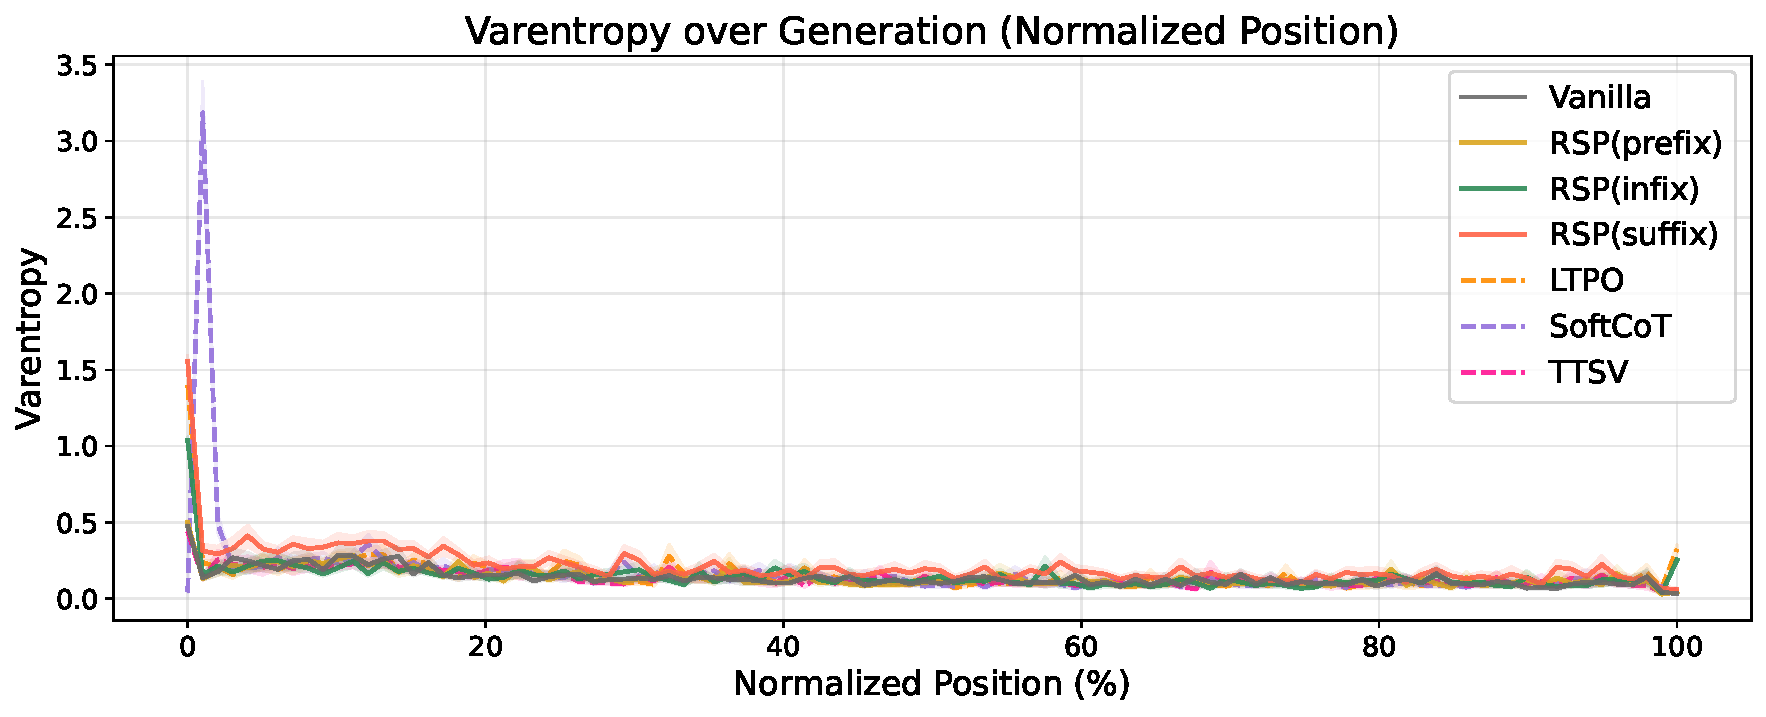
\includegraphics[width=0.85\textwidth]{img/entropy/full_varentropy.pdf}
  \caption{Mean entropy (top), top-1 probability (middle), and varentropy (bottom) over the full normalized generation trajectory (0--100\%). Averaged over MATH-500, shading indicates $\pm$1 SEM. Solid lines: RSP variants and the baseline. Dashed lines: existing soft prompt methods. All methods converge after the initial stage.}
  \label{fig:app_full_entropy}
\end{figure}

\iffalse
% =====================================================================
% Additional Semantic Diversity Analysis: hidden for current draft.
% Figure 2 in the main text was removed because the cluster analysis
% sometimes surfaces language artifacts that may be confused with
% reasoning-trajectory diversity. Restore when this confound is resolved.
% =====================================================================
\clearpage
\section{Additional Semantic Diversity Analysis}\label{app:semantic}

This appendix complements the semantic diversity results reported in Section~\ref{sec:diversity}. We include per-problem t-SNE plots across a broader set of problems.

\begin{figure}[ht]
  \centering
  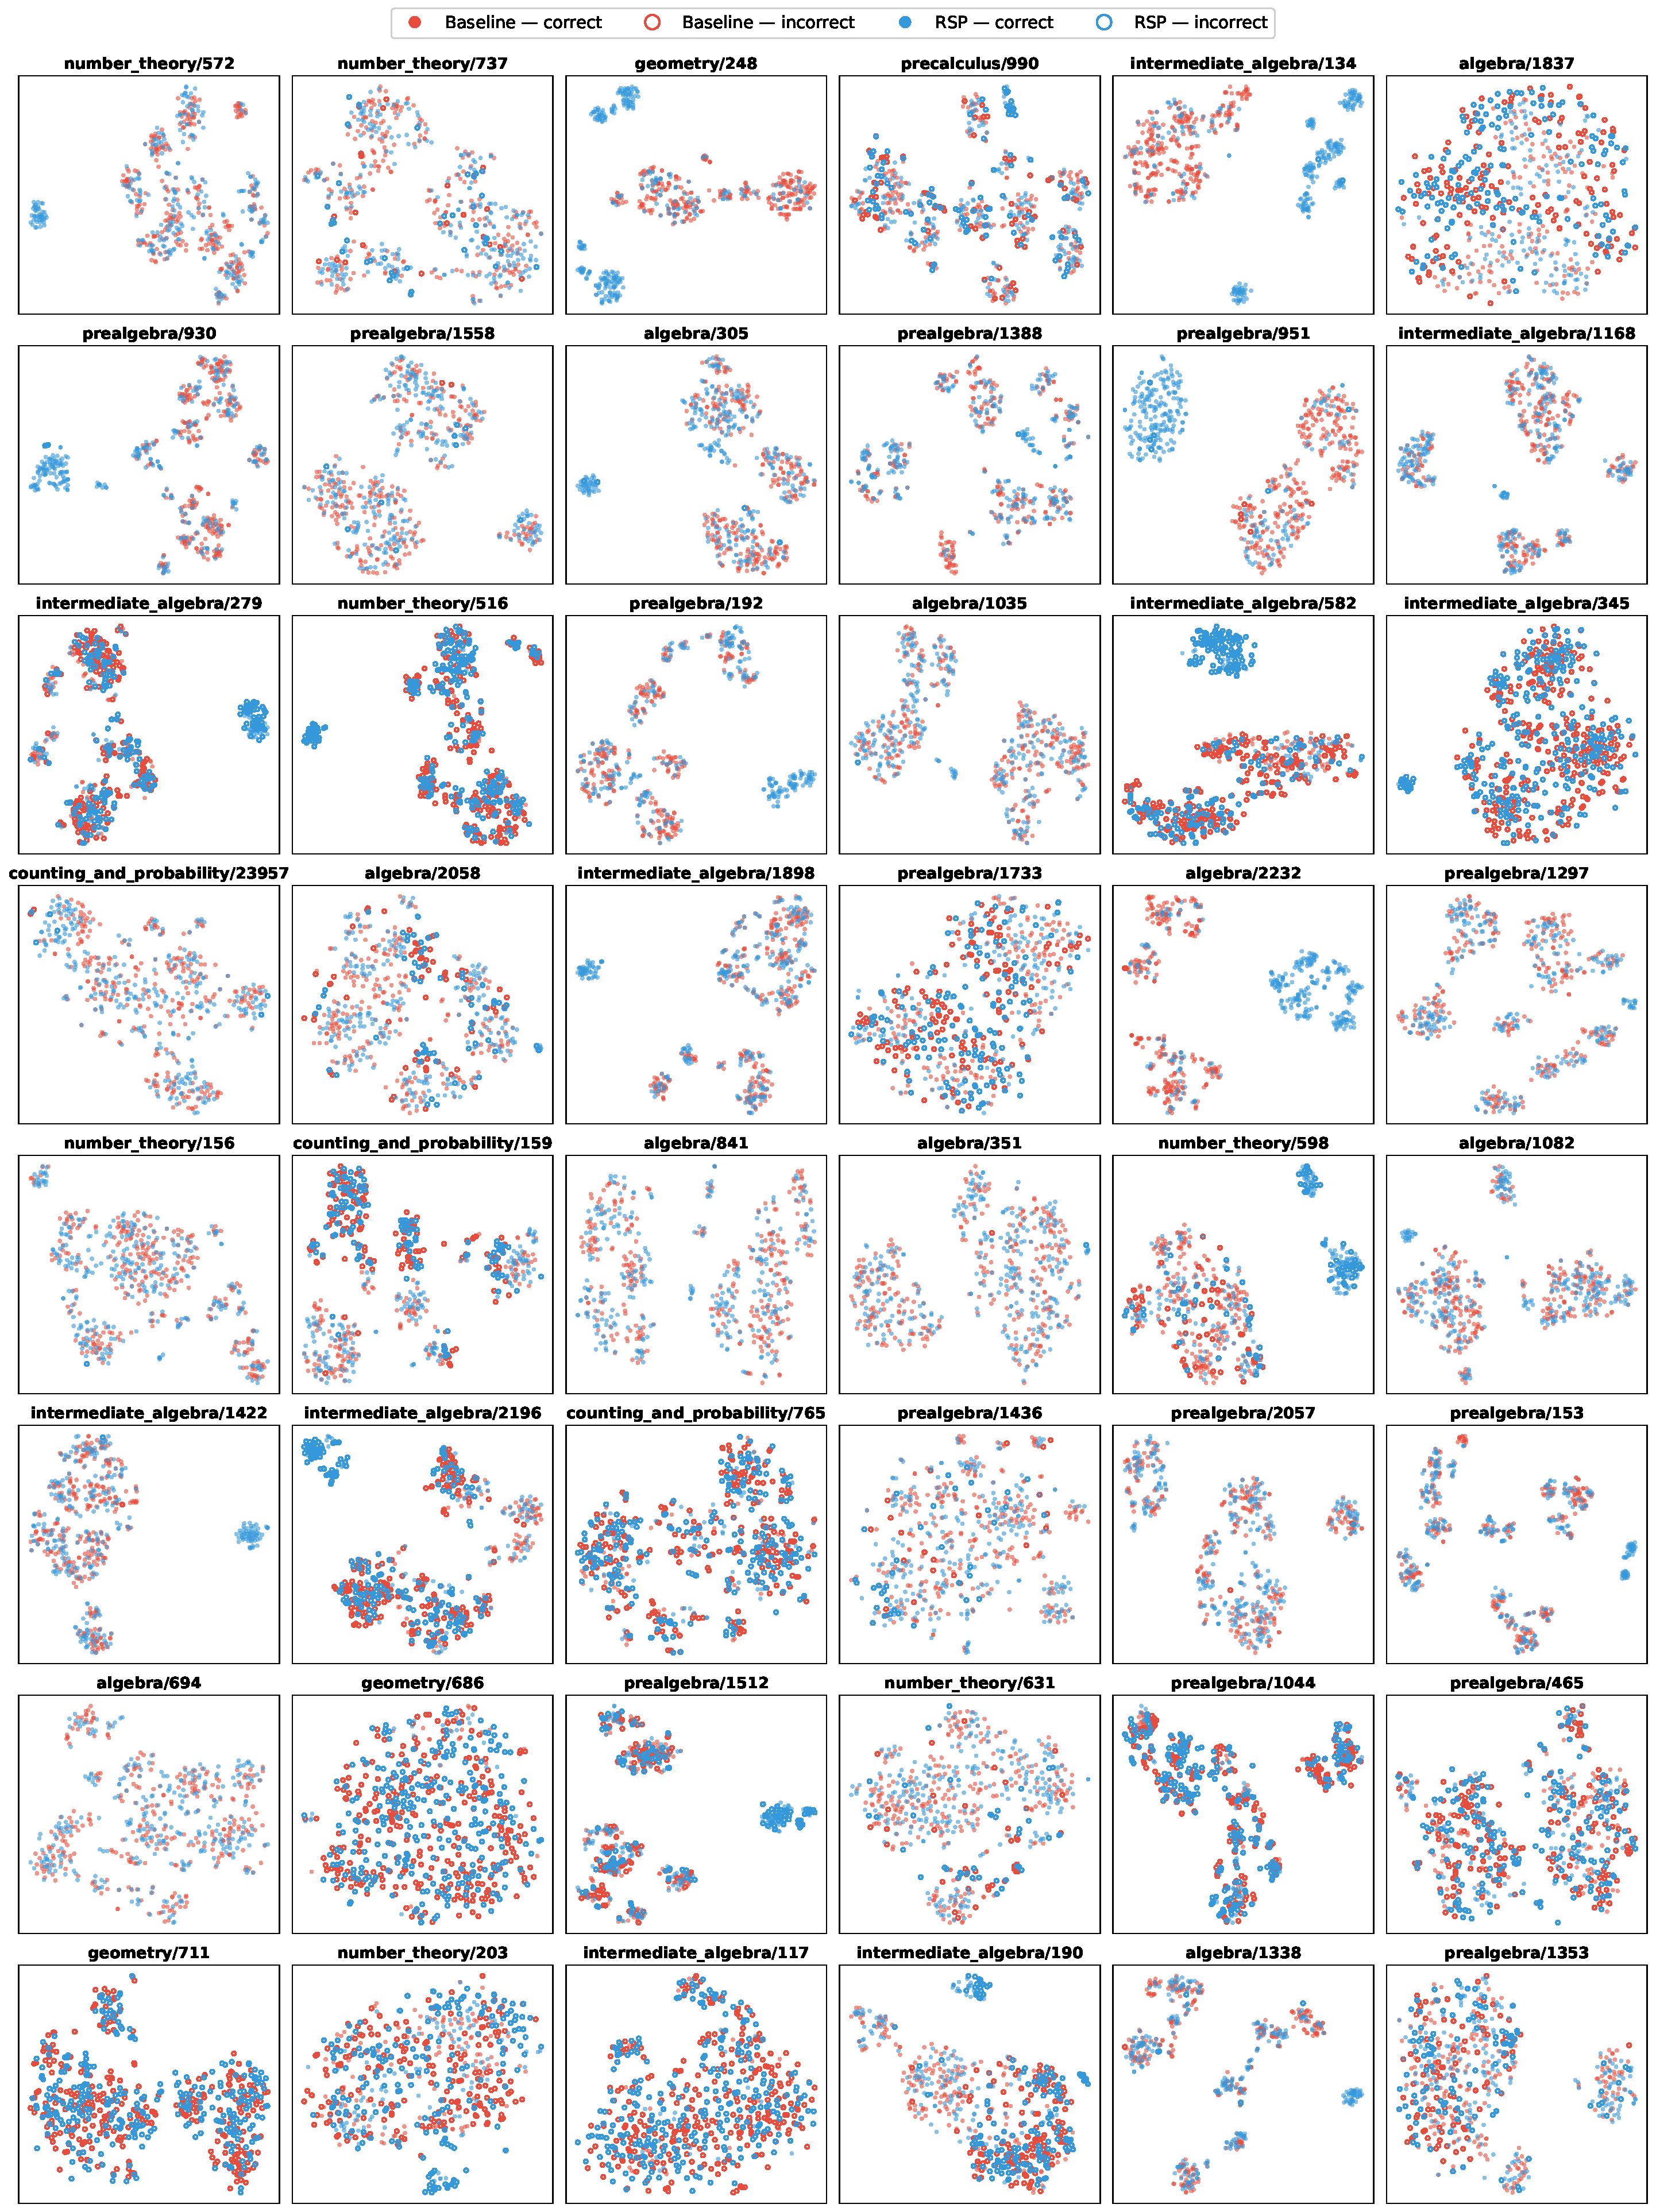
\includegraphics[width=\textwidth,height=0.75\textheight,keepaspectratio]{img/diversity/appendix_tsne_grid.pdf}
  \caption{t-SNE projections of BGE-M3 embeddings for 48 out of the 64 evaluated MATH-500 problems (6$\times$8 grid). Each subplot shows 300 baseline (red) and 300 RSP suffix (blue) samples under $\tau=1.0$ with Qwen2.5-Math-1.5B-Instruct; filled markers denote correct answers and open markers denote incorrect. Subplot titles indicate \texttt{subject/problem\_id}. Across most problems, RSP trajectories spread across multiple distinct regions while baseline samples concentrate in a single dominant cluster.}
  \label{fig:app_tsne_grid}
\end{figure}
\fi

\clearpage
\section{Token-Level Distribution Metrics}\label{app:token_metrics}

This appendix provides formal definitions for the three metrics used in the Token-level analysis of Section~\ref{sec:diversity}. Let $P_{\text{base}}$ denote the baseline next-token distribution at $\tau=1.0$ and $P_{\text{target}}$ the candidate distribution being compared (e.g., the baseline at $\tau=2.0$ or RSP at $\tau=1.0$). All metrics are computed analytically from saved logits at the first generation step.

\paragraph{Spearman rank correlation.}
Spearman's $\rho$ is the Pearson correlation coefficient between the token ranks of two distributions:
\begin{equation}
\rho \;=\; \mathrm{Pearson}\!\left(\mathrm{rank}(P_{\text{target}}),\; \mathrm{rank}(P_{\text{base}})\right).
\end{equation}
Because temperature scaling $P^{(\tau)} \propto P^{1/\tau}$ is a strictly monotone transform, the rank order of tokens is preserved exactly, so $\rho = 1$ for any $\tau > 0$ as a mathematical identity. Any value $\rho < 1$ therefore indicates rank reorganization beyond what temperature scaling can produce.

\paragraph{Mass outside top-$K$.}
Let $\mathrm{TopK}(P_{\text{base}})$ be the set of $K$ tokens with the highest probability under $P_{\text{base}}$. The probability mass that the candidate distribution places \emph{outside} this set is
\begin{equation}
\mathrm{MassOutside}_K \;=\; 1 - \sum_{t \in \mathrm{TopK}(P_{\text{base}})} P_{\text{target}}(t).
\end{equation}
This directly measures support expansion: how much probability the candidate assigns to tokens that are not in the baseline's preferred set. Reported values use $K = 10$.

\paragraph{Jensen--Shannon divergence.}
The symmetrized, bounded version of Kullback--Leibler divergence:
\begin{equation}
\mathrm{JS}(P, Q) \;=\; \tfrac{1}{2}\,\mathrm{KL}(P \,\|\, M) + \tfrac{1}{2}\,\mathrm{KL}(Q \,\|\, M), \qquad M = \tfrac{1}{2}(P + Q).
\end{equation}
We use base-2 logarithms so that $\mathrm{JS} \in [0, 1]$. Tokens absent from the stored top-100 are assigned a sentinel logit ($-10^9$) before softmax, which is negligible for our setting since the top-5 covers more than $99.9\%$ of the probability mass.

\clearpage
\section{Proofs for Energy-Theoretic Analysis}\label{app:proofs}

% [본문 문단 2, 3에 대한 증명]
% Hopfield energy의 smoothness로부터 매 layer에서 energy가 단조 감소함을 보이고,
% 이를 통해 perturbation 없는 forward pass가 local minimum에 갇힘을 증명
\subsection{Deterministic Trapping}

\begin{lemma}[Descent lemma]\label{lem:descent}
If $E$ is $L_E$-smooth and $\eta \leq 1/L_E$, then $E(\boldsymbol{\sigma}^{\mathrm{new}}) \leq E(\boldsymbol{\sigma}) - \frac{\eta}{2}\|\nabla E(\boldsymbol{\sigma})\|^2$.
\end{lemma}
\begin{proof}
By $L_E$-smoothness, $E(\boldsymbol{\sigma} - \eta \nabla E) \leq E(\boldsymbol{\sigma}) - \eta \|\nabla E\|^2 + \frac{L_E \eta^2}{2}\|\nabla E\|^2 = E(\boldsymbol{\sigma}) - \eta(1 - \frac{L_E \eta}{2})\|\nabla E\|^2$. Since $\eta \leq 1/L_E$, we have $L_E \eta / 2 \leq 1/2$, giving $E(\boldsymbol{\sigma}^{\mathrm{new}}) \leq E(\boldsymbol{\sigma}) - \frac{\eta}{2}\|\nabla E\|^2$.
\end{proof}

\begin{theorem}[Deterministic trapping]\label{thm:trapping_proof}
Without perturbation, the forward pass converges to the local minimum $\boldsymbol{\sigma}^*$ in the basin of attraction of $\boldsymbol{\sigma}^{(0)}$, which may satisfy $E(\boldsymbol{\sigma}^*) > E(\boldsymbol{\sigma}_g^*)$.
\end{theorem}
\begin{proof}
Lemma~\ref{lem:descent} guarantees monotone energy decrease at each layer: $E(\boldsymbol{\sigma}^{(l+1)}) \leq E(\boldsymbol{\sigma}^{(l)})$. Since $E$ is bounded below (the quadratic term dominates), the sequence $\{E(\boldsymbol{\sigma}^{(l)})\}$ converges, implying $\|\nabla E(\boldsymbol{\sigma}^{(l)})\| \to 0$ and convergence to a critical point. Deterministic dynamics follow a unique trajectory from $\boldsymbol{\sigma}^{(0)}$ and cannot cross energy barriers to reach minima in other basins.
\end{proof}

% [본문 문단 5 메커니즘 1에 대한 증명]
% RSP perturbation term의 expectation, covariance, bias-to-variance ratio를 유도
% bias가 negligible함을 보여 Langevin-like 해석을 정당화
\subsection{Properties of the RSP-Induced Perturbation}\label{app:rsp_noise}

\paragraph{Decomposition of attention output.}
The attention update with $n$ real keys and $k$ random keys can be decomposed as
\begin{equation}
\mathbf{x}_i^{(l+1)} = (1 - w_{r,i}^{(l)}) \, \tilde{\mathbf{x}}_i^{(l+1)} + \boldsymbol{\eta}_i^{(l)},
\end{equation}
where
\begin{equation}
\tilde{\mathbf{x}}_i^{(l+1)} = \sum_{j=1}^{n} \tilde{\alpha}_{ij}^{(l)} \mathbf{v}_j^{(l)}, \quad \tilde{\alpha}_{ij}^{(l)} = \frac{\alpha_{ij}^{(l)}}{1 - w_{r,i}^{(l)}},
\end{equation}
and
\begin{equation}
\boldsymbol{\eta}_i^{(l)} = \sum_{j=1}^{k} \alpha_{i,n+j}^{(l)} \mathbf{v}_{r_j}^{(l)}.
\end{equation}

We now analyze the properties of the perturbation term $\boldsymbol{\eta}_i^{(l)}$.

\paragraph{Conditional expectation.}
Conditioned on the attention weights, we have
\begin{equation}
\mathbb{E}\!\left[\boldsymbol{\eta}_i^{(l)} \mid \alpha^{(l)}\right] = \mu_E \, w_{r,i}^{(l)},
\end{equation}
where $w_{r,i}^{(l)} := \sum_{j=1}^{k} \alpha_{i,n+j}^{(l)}$.

\paragraph{Conditional covariance.}
Assuming the random vectors are independent with covariance $\sigma_E^2 \mathbf{I}$,
\begin{equation}
\mathrm{Cov}\!\left(\boldsymbol{\eta}_i^{(l)} \mid \alpha^{(l)}\right) = \sigma_E^2 \sum_{j=1}^{k} (\alpha_{i,n+j}^{(l)})^2 \, \mathbf{I}.
\end{equation}
Using $\sum_j \alpha_j^2 \le (\sum_j \alpha_j)^2$, we obtain
\begin{equation}
\mathrm{Cov}\!\left(\boldsymbol{\eta}_i^{(l)} \mid \alpha^{(l)}\right) \preceq \sigma_E^2 (w_{r,i}^{(l)})^2 \, \mathbf{I}.
\end{equation}

\paragraph{Bias-to-variance ratio.}
The ratio between the mean and standard deviation is bounded by
\begin{equation}
\frac{\|\mathbb{E}[\boldsymbol{\eta}_i^{(l)} \mid \alpha^{(l)}]\|}{\sqrt{\mathrm{Var}(\boldsymbol{\eta}_i^{(l)} \mid \alpha^{(l)})}} \le \frac{|\mu_E|}{\sigma_E}.
\end{equation}
Empirically, $|\mu_E|/\sigma_E \ll 1$, implying that the stochastic component dominates the bias.

\paragraph{Empirical verification.}
Table~\ref{tab:embed_stats} reports the embedding matrix statistics for all models used in our experiments.

\begin{table}[ht]
\centering
\caption{Embedding matrix statistics. $|\mu_E|/\sigma_E < 0.02$ across all models.}
\label{tab:embed_stats}
\footnotesize
\renewcommand{\arraystretch}{0.9}
\begin{tabular}{lccc}
\toprule
\textbf{Model} & $\mu_E$ & $\sigma_E$ & $|\mu_E|/\sigma_E$ \\
\midrule
LLaMA-3.1-8B-Instruct & 0.00002 & 0.01057 & 0.002 \\
Qwen2.5-Math-7B-Instruct & $-$0.00002 & 0.01647 & 0.001 \\
Qwen2.5-Math-1.5B-Instruct & 0.00019 & 0.01585 & 0.012 \\
Qwen2.5-Math-7B & $-$0.00003 & 0.01842 & 0.001 \\
Qwen2.5-Math-1.5B & 0.00038 & 0.02990 & 0.013 \\
\bottomrule
\end{tabular}
\end{table}

\paragraph{Implication.}
Therefore, the perturbation behaves as approximately zero-mean noise whose magnitude is controlled by $w_{r,i}^{(l)}$, justifying the Langevin-like interpretation in the main text.

% [본문 문단 6에 대한 증명]
% attention decay bound: softmax 정규화에서 real key의 exponential sum을 lower bound하여 유도
\subsection{Attention Decay Bound}

\begin{theorem}[Attention decay]\label{thm:decay_proof}
The total attention on random tokens satisfies
\begin{equation}
w_{r,i}^{(l)} \leq \frac{k}{k + n \cdot \exp(\Delta_i^{(l)} / \sqrt{d})},
\end{equation}
where $\Delta_i^{(l)} := \min_{j \in [n]} \mathbf{q}_i^\top \mathbf{k}_j - \max_{j' \in [k]} \mathbf{q}_i^\top \mathbf{k}_{r_{j'}}$ is the real-vs-random logit gap.
\end{theorem}
\begin{proof}
Let $s_j = \mathbf{q}_i^\top \mathbf{k}_j / \sqrt{d}$ for real keys and $s_{r_{j'}} = \mathbf{q}_i^\top \mathbf{k}_{r_{j'}} / \sqrt{d}$ for random keys. By definition of $\Delta_i^{(l)}$, each real key satisfies $s_j \geq \Delta_i^{(l)}/\sqrt{d} + s_{r,\max}$ where $s_{r,\max} = \max_{j'} s_{r_{j'}}$. Therefore $\exp(s_j) \geq \exp(\Delta_i^{(l)}/\sqrt{d}) \cdot \exp(s_{r,\max})$ for every real key. Summing over $n$ real keys:
\begin{equation}
\sum_{j=1}^{n} \exp(s_j) \geq n \cdot \exp(\Delta_i^{(l)}/\sqrt{d}) \cdot \exp(s_{r,\max}) \geq n \cdot \exp(\Delta_i^{(l)}/\sqrt{d}) \cdot \frac{1}{k}\sum_{j'=1}^{k} \exp(s_{r_{j'}}).
\end{equation}
The total attention on random tokens is $w_{r,i}^{(l)} = \sum_{j'} \exp(s_{r_{j'}}) / (\sum_j \exp(s_j) + \sum_{j'} \exp(s_{r_{j'}}))$. Substituting the lower bound on the real-key sum and letting $R = \sum_{j'} \exp(s_{r_{j'}})$:
\begin{equation}
w_{r,i}^{(l)} = \frac{R}{\sum_j \exp(s_j) + R} \leq \frac{R}{n \cdot \exp(\Delta_i^{(l)}/\sqrt{d}) \cdot R/k + R} = \frac{k}{k + n \cdot \exp(\Delta_i^{(l)}/\sqrt{d})}.
\end{equation}
\end{proof}

% [본문 Section 4.2 (Output Distribution Shift and Exploration) 에 대한 증명]
% autoregressive formulation, local linearization, Proposition 1/2 증명, trajectory-level implications
\subsection{Proofs for Output Distribution Shift}

\subsubsection{Autoregressive Formulation}

In autoregressive decoding, the joint distribution over a sequence $y_{1:T}$ factorizes as
\[
\Pr(y_{1:T} \mid x) = \prod_{t=1}^T p(y_t \mid x, y_{<t}),
\]
where each step is governed by a prefix-conditioned distribution. Any perturbation introduced by RSP affects generation through a sequence of local changes to $p(y_t \mid x, y_{<t})$, rather than a single global distribution.

\subsubsection{Local Linearization of Logits under RSP}

Let $h$ denote the random soft prompt. We model the perturbed logits as a function $z_i(h)$, assuming local smoothness in a neighborhood of $h=0$:
\[
z_i(h) = z_i(0) + \nabla_h z_i(0)^\top h + r_i(h),
\]
where $r_i(h) = O(\|h\|^2)$. Defining $a_i := \nabla_h z_i(0)$, we obtain the local linear approximation $z_i(h) \approx z_i + a_i^\top h$. This approximation is valid for sufficiently small $\|h\|$ and is used to characterize the direction of perturbation rather than exact logit values.

\subsubsection{Proof of Proposition 1 (Stochastic Ranking)}

\textit{If there exists a token pair $(i,j)$ such that $a_i \neq a_j$, then $0 < \Pr_h(z_i(h) > z_j(h)) < 1$.}

\begin{proof}
Under the local linear approximation, $z_i(h) - z_j(h) = (z_i - z_j) + (a_i - a_j)^\top h$. Let $b_{ij} := a_i - a_j \neq 0$. If $h \sim \mathcal{N}(0, \sigma^2 I)$, then $b_{ij}^\top h \sim \mathcal{N}(0, \sigma^2 \|b_{ij}\|^2)$, a non-degenerate Gaussian. The perturbed logit difference $\Delta_{ij}(h) := (z_i - z_j) + b_{ij}^\top h$ therefore has non-zero probability mass on both sides of zero: $0 < \Pr_h(\Delta_{ij}(h) > 0) < 1$.
\end{proof}

\subsubsection{On Proposition 2 (Support Expansion)}

Proposition 2 states that tokens outside the baseline top-$K$ set can enter the top-$K$ set under RSP with positive probability. Proposition 1 establishes that pairwise ranking between tokens becomes stochastic. Entering the top-$K$ set requires surpassing multiple tokens simultaneously, i.e., conditions of the form $z_i(h) > z_j(h)$ for all $j \in J$ where $J$ is a subset of higher-ranked tokens. Under the local linear model, these inequalities define a region in $h$-space. If this region has non-zero measure under the distribution of $h$, then top-$K$ entry occurs with positive probability. We interpret Proposition 2 as a support-expansion statement: RSP enables tokens that are effectively inaccessible under deterministic ranking to become reachable under stochastic perturbations.

\subsubsection{Trajectory-Level Implications}

Since autoregressive generation composes conditional distributions across steps, perturbations at early steps can lead to distinct trajectories. Let $\mathcal{R}_{k,K}(x)$ denote the set of trajectories containing at least one token outside the baseline top-$K$ set. If RSP increases the accessibility of such tokens at early steps, then the probability of sampling trajectories in $\mathcal{R}_{k,K}(x)$ increases under repeated sampling. This links local ranking perturbations to global trajectory diversity.

\clearpage
% ================================================================
\section{Attention Mass Analysis}\label{app:attention_mass}
% ================================================================

This appendix formalizes the per-token attention mass reported in Figure~\ref{fig:attention_mass} and the exclusion criteria applied to the reasoning span and the layer axis. For each of the 500 MATH-500 problems, a fresh RSP $\mathbf{H} \in \mathbb{R}^{L \times d}$ with $L = 10$ is sampled independently, so the reported heatmaps average over both problem variability and RSP-vector variability.

\subsection{Per-Token Attention Mass}

For each problem, we measure attention on the concatenated sequence $[\text{prompt}; \mathbf{H}; \text{generation}]$, where the generation is the trajectory produced by the same model under matching RSP injection. Let $\alpha^{(\ell, h)}_{i,j}$ denote the post-softmax attention weight at layer $\ell$, head $h$, from query position $i$ to key position $j$, satisfying $\sum_j \alpha^{(\ell, h)}_{i,j} = 1$ under the causal mask. Let $Q$ and $R$ denote the index sets of question and RSP tokens with sizes $|Q|$ and $|R| = L$, and let $H$ be the number of heads. The per-token attention mass that query $i$ directs to each group at layer $\ell$ is
\begin{equation}
\mathrm{PTM}_{Q}[\ell, i] = \frac{1}{|Q| H} \sum_{h=1}^{H} \sum_{j \in Q} \alpha^{(\ell, h)}_{i,j},
\qquad
\mathrm{PTM}_{R}[\ell, i] = \frac{1}{|R| H} \sum_{h=1}^{H} \sum_{j \in R} \alpha^{(\ell, h)}_{i,j}.
\label{eq:per_token_mass}
\end{equation}
Normalization by $|Q|$ and $|R|$ controls for group size, so both quantities express how much attention a single question (resp.\ RSP) token receives on average under the same softmax denominator. Question tokens thereby serve as a size-matched baseline that absorbs sequence-length effects common to both groups.

\subsection{Heatmap Aggregation}

We partition the layer indices and the reasoning position indices each into five equal-size bins $\{B_L^{(b)}\}_{b=1}^{5}$ and $\{B_P^{(b)}\}_{b=1}^{5}$. For sample $s$ and target group $\bullet \in \{Q, R\}$, the value in cell $(b_L, b_P)$ is
\begin{equation}
M^{(s)}_{\bullet}[b_L, b_P] = \frac{1}{|B_L^{(b_L)}| \cdot |B_P^{(b_P)}|} \sum_{\ell \in B_L^{(b_L)}} \sum_{i \in B_P^{(b_P)}} \mathrm{PTM}_{\bullet}[\ell, i].
\label{eq:binned_mass}
\end{equation}
Figure~\ref{fig:attention_mass} reports the sample average of Eq.~\eqref{eq:binned_mass} over the 500 valid samples.

\subsection{Excluding the \texttt{\textbackslash boxed\{\ldots\}} Span}

The reasoning position range terminates strictly before the final \texttt{\textbackslash boxed\{\ldots\}} span. Chain-of-thought outputs decompose into a \textit{text} (content) component and a \textit{pattern} (template) component that contribute independently to downstream performance \citep{madaan2022text}. The \texttt{\textbackslash boxed\{\ldots\}} wrapper is a canonical pattern: a short, stereotyped span whose role is to complete the answer format rather than to extend reasoning. Including it would therefore inject a template-driven attention signature unrelated to reasoning dynamics.

\subsection{Excluding the Final Two Layers}

The layer axis further excludes the last two transformer layers. Two well-documented properties of late layers, none specific to our setup, motivate this choice.

\paragraph{Output-projection specialization.}
Late-layer hidden states lie in an approximately linear relationship with vocabulary logits and therefore function as a progressive linear readout rather than as representation-transforming blocks \citep{belrose2023eliciting}. Consistently, late-layer feed-forward modules have been characterized as output-distribution shaping mechanisms \citep{geva2021transformer}. Attention in these layers therefore reflects output formation rather than reasoning computation.

\paragraph{Register-token hypothesis.}
Uninformative patch tokens in Vision Transformers have been shown to be repurposed as \textit{registers}: storage slots that absorb attention in deeper layers \citep{darcet2023vision}. Because RSPs share a similar profile as continuous tokens without pretrained semantic content, a similar repurposing in late transformer layers cannot be ruled out. Excluding the final two layers removes this potential register-induced confound from the reasoning-phase signal.

The two lines of evidence above identify known late-layer phenomena --- linear readout and potential register repurposing --- whose attention signatures are orthogonal to reasoning-phase dynamics. Removing the final two layers preempts their contamination of the reasoning-phase signal, yielding a principled, literature-grounded exclusion rather than a model-specific tuning decision.

\subsection{Additional Suffix Heatmaps}

Figure~\ref{fig:app_attention_additional} reports the same per-token RSP attention analysis under suffix injection for Qwen2.5-Math-1.5B-Instruct and LLaMA-3.1-8B-Instruct. For the late-layer reasons discussed above, the pattern does not generalize uniformly across every cell; nevertheless, the overall trend is consistent across both models: question-token attention varies broadly across layers, whereas RSP attention shows the layer-wise and sequence-wise decay predicted by Eq.~\eqref{eq:decay_main}.

\begin{figure}[ht]
  \centering
  \begin{subfigure}[b]{\textwidth}
    \centering
    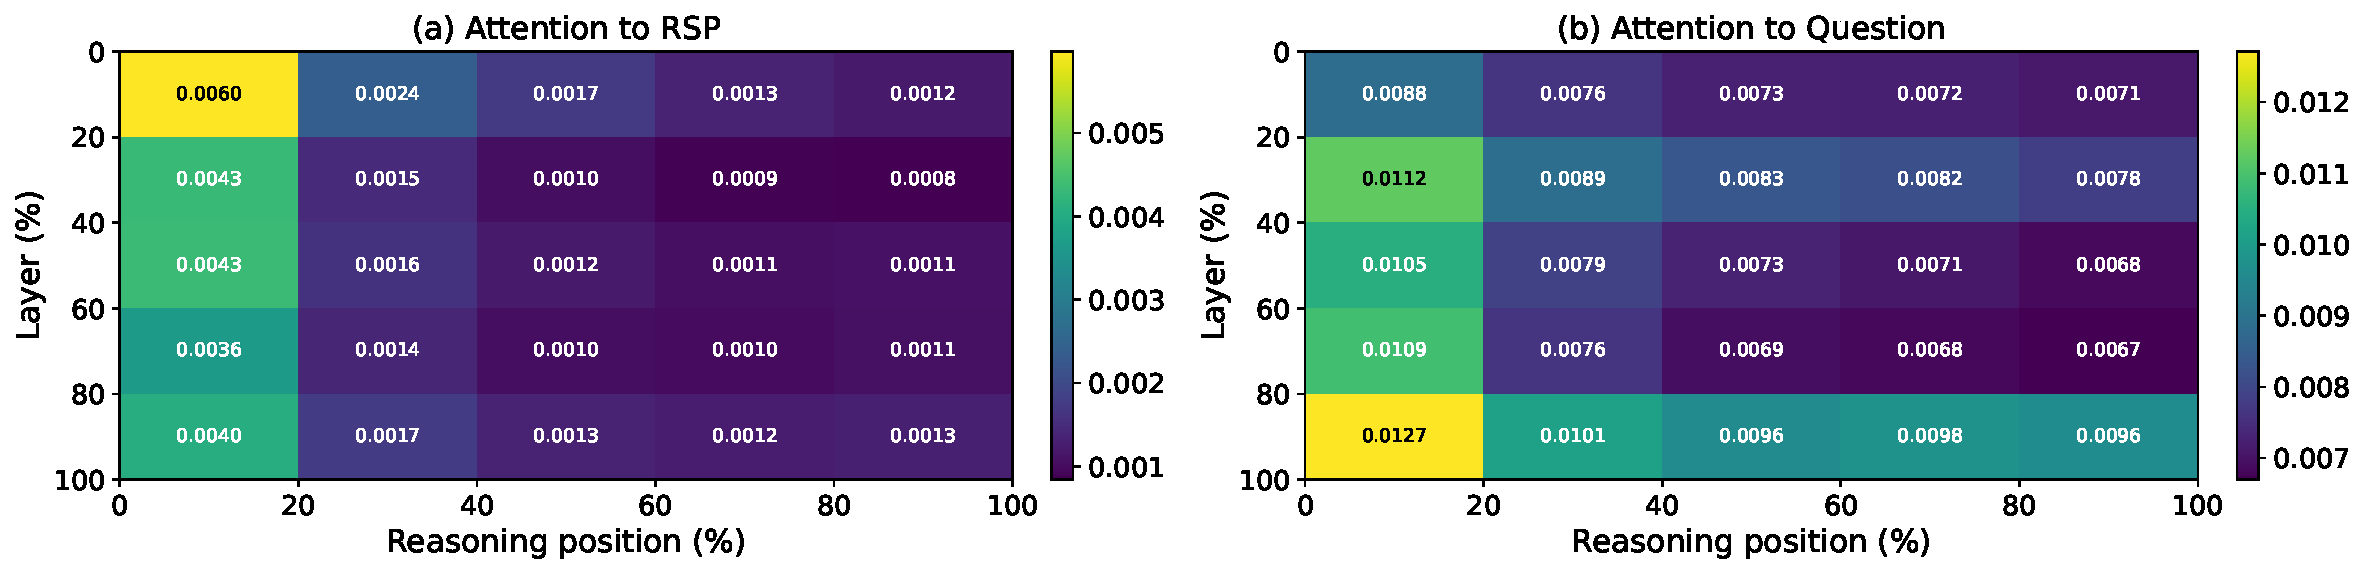
\includegraphics[width=\textwidth]{img/attention/heatmap_qwen1.5b_suffix.pdf}
    \caption{Qwen2.5-Math-1.5B-Instruct, suffix}
  \end{subfigure}
  \\[0.5em]
  \begin{subfigure}[b]{\textwidth}
    \centering
    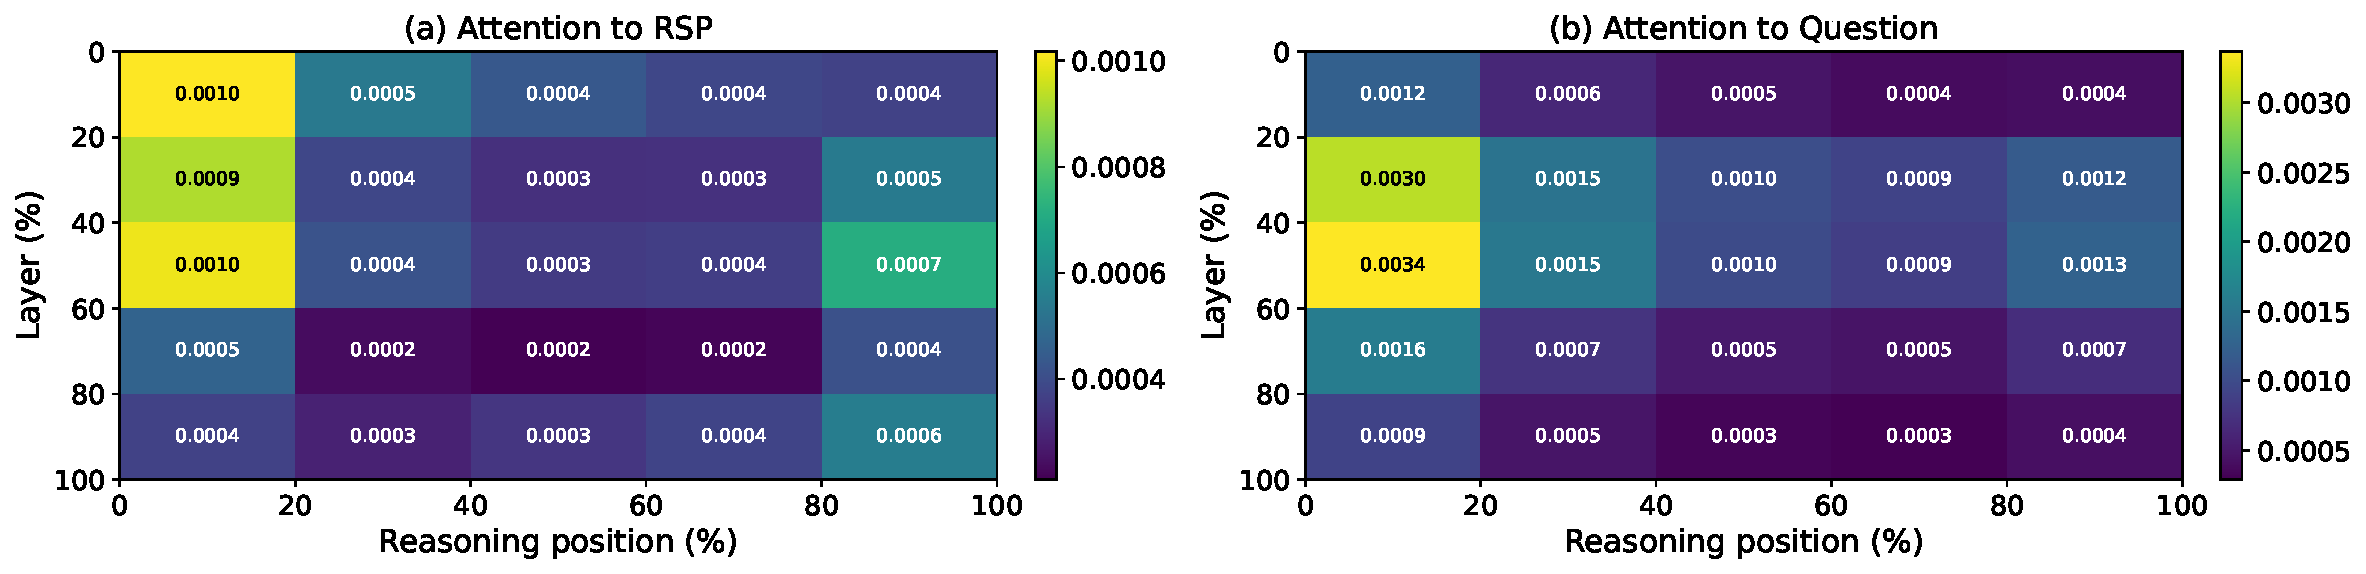
\includegraphics[width=\textwidth]{img/attention/heatmap_llama8b_suffix.pdf}
    \caption{LLaMA-3.1-8B-Instruct, suffix}
  \end{subfigure}
  \caption{Per-token RSP attention mass under suffix injection for the remaining two models (500 MATH-500 samples each). Axes and preprocessing match Figure~\ref{fig:attention_mass}: x-axis is reasoning position binned into five quantiles, y-axis is layer depth binned into five quantiles (top = shallow), color encodes the 500-sample mean per-token attention assigned to RSP tokens, and tokens inside \texttt{\textbackslash boxed\{\}} spans and the last two layers are excluded.}
  \label{fig:app_attention_additional}
\end{figure}

\clearpage
% ================================================================
\section{GRPO Formulation}\label{app:grpo}
% ================================================================

For a given prompt $q$, the behavior policy $\pi_{\theta_{\text{old}}}$ samples a group of $G$ responses $\{o_i\}_{i=1}^G$ with corresponding rewards $\{R_i\}_{i=1}^G$. The advantage of each response is computed by normalizing the group-level rewards:
\begin{equation}
  \hat{A}_{i,t} = \frac{R_i - \text{mean}(\{R_i\}_{i=1}^G)}{\text{std}(\{R_i\}_{i=1}^G)}.
\end{equation}
The policy is updated via a clipped objective with a KL penalty:
\begin{equation}
  \mathcal{J}_{\text{GRPO}}(\theta) = \mathbb{E} \left[ \frac{1}{G} \sum_{i=1}^{G} \frac{1}{|o_i|} \sum_{t=1}^{|o_i|} \left( \min\left( r_{i,t} \hat{A}_{i,t},\; \text{clip}(r_{i,t}, 1\!-\!\varepsilon, 1\!+\!\varepsilon)\, \hat{A}_{i,t} \right) - \beta D_{\text{KL}}(\pi_\theta \| \pi_{\text{ref}}) \right) \right],
\end{equation}
where $r_{i,t} = \pi_\theta(o_{i,t} \mid q, o_{i,<t}) / \pi_{\theta_{\text{old}}}(o_{i,t} \mid q, o_{i,<t})$ is the importance sampling ratio, $\varepsilon$ is the clipping range, and $\beta$ controls the strength of the KL penalty against the reference policy $\pi_{\text{ref}}$.

\clearpage
% ================================================================
\section{Broader Impacts}\label{app:broader_impacts}
% ================================================================

This work provides empirical and theoretical analysis of how random embedding injection affects the reasoning behavior of large language models. The contributions are primarily foundational, with potential downstream implications for reinforcement learning-based post-training of reasoning models such as GRPO.

\paragraph{Positive impacts.}
RSP-induced trajectory diversity could improve the sample efficiency of RL-based LLM post-training by providing richer learning signals within group-relative advantage estimation. This has the potential to reduce compute costs associated with alignment and reasoning-oriented fine-tuning, making such methods more accessible to research groups with limited resources.

\paragraph{Potential concerns.}
Methods that expand the effective output support of LLMs may increase the reachability of low-probability tokens, which includes both desirable alternative reasoning paths and potentially unsafe or off-distribution outputs. Practitioners applying RSP in production systems should combine it with existing safety filtering and alignment mechanisms rather than treating it as a standalone diversity source.

\paragraph{Limitations on impact scope.}
Since this work focuses on analysis rather than deploying a new model or dataset, the direct societal impact is limited. The broader implications described above are contingent on future work integrating RSP into applied training pipelines.
